\renewcommand{\leveltopI}{-15cm + \leveltop}
\renewcommand{\leveltopII}{-15cm + \leveltopI}
\renewcommand{\leveltopIII}{-15cm + \leveltopII}
\renewcommand{\leveltopIIII}{-15cm + \leveltopIII}
\renewcommand{\leveltopIIIII}{-15cm + \leveltopIIII}
\renewcommand{\leveltopIIIIII}{-15cm + \leveltopIIIII}
\renewcommand{\leveltopIIIIIII}{-15cm + \leveltopIIIIII}
\renewcommand{\leveltopIIIIIIII}{-15cm + \leveltopIIIIIII}
\renewcommand{\leveltopIIIIIIIII}{-15cm + \leveltopIIIIIIII}
\renewcommand{\leveltopIIIIIIIIII}{-15cm + \leveltopIIIIIIIII}
\begin{tikzpicture}[scale=.2, anchor=south]
\begin{scope}[yshift=\leveltopI cm]
\matrix (line1) [column sep=1cm] {
\node[draw=black, rectangle split,  rectangle split parts=4] (sn0x250ba90){
\footnotesize{1}
\nodepart{two}
\begin{tikzpicture}[scale=.2]
\node[circle, scale=0.75, fill] (tid0) at (4.5,1.5){};
\node[circle, scale=0.75, fill] (tid1) at (3,3){};
\node[circle, scale=0.75, fill] (tid4) at (1.5,4.5){};
\node[circle, scale=0.75, fill, red] (tid8) at (0.75,6){};
\node[circle, scale=0.75, fill, red] (tid9) at (2.25,6){};
\draw[](tid4) -- (tid8);
\draw[](tid4) -- (tid9);
\node[circle, scale=0.75, fill] (tid5) at (3.75,4.5){};
\node[circle, scale=0.75, fill] (tid6) at (5.25,4.5){};
\draw[](tid1) -- (tid4);
\draw[](tid1) -- (tid5);
\draw[](tid1) -- (tid6);
\node[circle, scale=0.75, fill] (tid2) at (6.75,3){};
\node[circle, scale=0.75, fill, red] (tid7) at (6.75,4.5){};
\draw[](tid2) -- (tid7);
\node[circle, scale=0.75, fill] (tid3) at (8.25,3){};
\draw[](tid0) -- (tid1);
\draw[](tid0) -- (tid2);
\draw[](tid0) -- (tid3);
\end{tikzpicture}
\nodepart{three}
\footnotesize{5.36185}
\nodepart{four}
\footnotesize{$33\:67$}
};
 & 
\\
};
\end{scope}
\begin{scope}[yshift=\leveltopII cm]
\matrix (line2) [column sep=1cm] {
\node[draw=black, rectangle split,  rectangle split parts=4] (sn0x250d5a0){
\footnotesize{0.333333}
\nodepart{two}
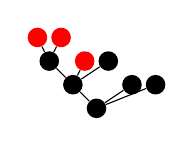
\begin{tikzpicture}[scale=.2]
\node[circle, scale=0.75, fill] (tid0) at (4.5,1.5){};
\node[circle, scale=0.75, fill] (tid1) at (3,3){};
\node[circle, scale=0.75, fill] (tid4) at (1.5,4.5){};
\node[circle, scale=0.75, fill, red] (tid7) at (0.75,6){};
\node[circle, scale=0.75, fill, red] (tid8) at (2.25,6){};
\draw[](tid4) -- (tid7);
\draw[](tid4) -- (tid8);
\node[circle, scale=0.75, fill, red] (tid5) at (3.75,4.5){};
\node[circle, scale=0.75, fill] (tid6) at (5.25,4.5){};
\draw[](tid1) -- (tid4);
\draw[](tid1) -- (tid5);
\draw[](tid1) -- (tid6);
\node[circle, scale=0.75, fill] (tid2) at (6.75,3){};
\node[circle, scale=0.75, fill] (tid3) at (8.25,3){};
\draw[](tid0) -- (tid1);
\draw[](tid0) -- (tid2);
\draw[](tid0) -- (tid3);
\end{tikzpicture}
\nodepart{three}
\footnotesize{5.10151}
\nodepart{four}
\footnotesize{$33\:67$}
};
 & 
\node[draw=black, rectangle split,  rectangle split parts=4] (sn0x250c380){
\footnotesize{0.666667}
\nodepart{two}
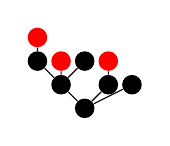
\begin{tikzpicture}[scale=.2]
\node[circle, scale=0.75, fill] (tid0) at (3.75,1.5){};
\node[circle, scale=0.75, fill] (tid1) at (2.25,3){};
\node[circle, scale=0.75, fill] (tid4) at (0.75,4.5){};
\node[circle, scale=0.75, fill, red] (tid8) at (0.75,6){};
\draw[](tid4) -- (tid8);
\node[circle, scale=0.75, fill, red] (tid5) at (2.25,4.5){};
\node[circle, scale=0.75, fill] (tid6) at (3.75,4.5){};
\draw[](tid1) -- (tid4);
\draw[](tid1) -- (tid5);
\draw[](tid1) -- (tid6);
\node[circle, scale=0.75, fill] (tid2) at (5.25,3){};
\node[circle, scale=0.75, fill, red] (tid7) at (5.25,4.5){};
\draw[](tid2) -- (tid7);
\node[circle, scale=0.75, fill] (tid3) at (6.75,3){};
\draw[](tid0) -- (tid1);
\draw[](tid0) -- (tid2);
\draw[](tid0) -- (tid3);
\end{tikzpicture}
\nodepart{three}
\footnotesize{4.99203}
\nodepart{four}
\footnotesize{$33\:33\:33$}
};
 & 
\\
};
\end{scope}
\begin{scope}[yshift=\leveltopIII cm]
\matrix (line3) [column sep=1cm] {
\node[draw=black, rectangle split,  rectangle split parts=4] (sn0x250de90){
\footnotesize{0.111111}
\nodepart{two}
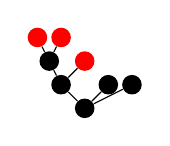
\begin{tikzpicture}[scale=.2]
\node[circle, scale=0.75, fill] (tid0) at (3.75,1.5){};
\node[circle, scale=0.75, fill] (tid1) at (2.25,3){};
\node[circle, scale=0.75, fill] (tid4) at (1.5,4.5){};
\node[circle, scale=0.75, fill, red] (tid6) at (0.75,6){};
\node[circle, scale=0.75, fill, red] (tid7) at (2.25,6){};
\draw[](tid4) -- (tid6);
\draw[](tid4) -- (tid7);
\node[circle, scale=0.75, fill, red] (tid5) at (3.75,4.5){};
\draw[](tid1) -- (tid4);
\draw[](tid1) -- (tid5);
\node[circle, scale=0.75, fill] (tid2) at (5.25,3){};
\node[circle, scale=0.75, fill] (tid3) at (6.75,3){};
\draw[](tid0) -- (tid1);
\draw[](tid0) -- (tid2);
\draw[](tid0) -- (tid3);
\end{tikzpicture}
\nodepart{three}
\footnotesize{4.8786}
\nodepart{four}
\footnotesize{$33\:67$}
};
 & 
\node[draw=black, rectangle split,  rectangle split parts=4] (sn0x250d150){
\footnotesize{0.444444}
\nodepart{two}
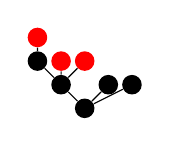
\begin{tikzpicture}[scale=.2]
\node[circle, scale=0.75, fill] (tid0) at (3.75,1.5){};
\node[circle, scale=0.75, fill] (tid1) at (2.25,3){};
\node[circle, scale=0.75, fill] (tid4) at (0.75,4.5){};
\node[circle, scale=0.75, fill, red] (tid7) at (0.75,6){};
\draw[](tid4) -- (tid7);
\node[circle, scale=0.75, fill, red] (tid5) at (2.25,4.5){};
\node[circle, scale=0.75, fill, red] (tid6) at (3.75,4.5){};
\draw[](tid1) -- (tid4);
\draw[](tid1) -- (tid5);
\draw[](tid1) -- (tid6);
\node[circle, scale=0.75, fill] (tid2) at (5.25,3){};
\node[circle, scale=0.75, fill] (tid3) at (6.75,3){};
\draw[](tid0) -- (tid1);
\draw[](tid0) -- (tid2);
\draw[](tid0) -- (tid3);
\end{tikzpicture}
\nodepart{three}
\footnotesize{4.71296}
\nodepart{four}
\footnotesize{$67\:33$}
};
 & 
\node[draw=black, rectangle split,  rectangle split parts=4] (sn0x2512830){
\footnotesize{0.222222}
\nodepart{two}
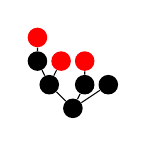
\begin{tikzpicture}[scale=.2]
\node[circle, scale=0.75, fill] (tid0) at (3,1.5){};
\node[circle, scale=0.75, fill] (tid1) at (1.5,3){};
\node[circle, scale=0.75, fill] (tid4) at (0.75,4.5){};
\node[circle, scale=0.75, fill, red] (tid7) at (0.75,6){};
\draw[](tid4) -- (tid7);
\node[circle, scale=0.75, fill, red] (tid5) at (2.25,4.5){};
\draw[](tid1) -- (tid4);
\draw[](tid1) -- (tid5);
\node[circle, scale=0.75, fill] (tid2) at (3.75,3){};
\node[circle, scale=0.75, fill, red] (tid6) at (3.75,4.5){};
\draw[](tid2) -- (tid6);
\node[circle, scale=0.75, fill] (tid3) at (5.25,3){};
\draw[](tid0) -- (tid1);
\draw[](tid0) -- (tid2);
\draw[](tid0) -- (tid3);
\end{tikzpicture}
\nodepart{three}
\footnotesize{4.73225}
\nodepart{four}
\footnotesize{$33\:33\:33$}
};
 & 
\node[draw=black, rectangle split,  rectangle split parts=4] (sn0x2512ab0){
\footnotesize{0.222222}
\nodepart{two}
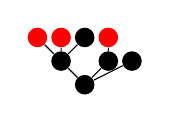
\begin{tikzpicture}[scale=.2]
\node[circle, scale=0.75, fill] (tid0) at (3.75,1.5){};
\node[circle, scale=0.75, fill] (tid1) at (2.25,3){};
\node[circle, scale=0.75, fill, red] (tid4) at (0.75,4.5){};
\node[circle, scale=0.75, fill, red] (tid5) at (2.25,4.5){};
\node[circle, scale=0.75, fill] (tid6) at (3.75,4.5){};
\draw[](tid1) -- (tid4);
\draw[](tid1) -- (tid5);
\draw[](tid1) -- (tid6);
\node[circle, scale=0.75, fill] (tid2) at (5.25,3){};
\node[circle, scale=0.75, fill, red] (tid7) at (5.25,4.5){};
\draw[](tid2) -- (tid7);
\node[circle, scale=0.75, fill] (tid3) at (6.75,3){};
\draw[](tid0) -- (tid1);
\draw[](tid0) -- (tid2);
\draw[](tid0) -- (tid3);
\end{tikzpicture}
\nodepart{three}
\footnotesize{4.53086}
\nodepart{four}
\footnotesize{$33\:67$}
};
 & 
\\
};
\end{scope}
\begin{scope}[yshift=\leveltopIIII cm]
\matrix (line4) [column sep=1cm] {
\node[draw=black, rectangle split,  rectangle split parts=4] (sn0x250dd40){
\footnotesize{0.037037}
\nodepart{two}
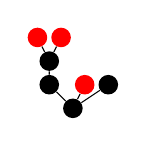
\begin{tikzpicture}[scale=.2]
\node[circle, scale=0.75, fill] (tid0) at (3,1.5){};
\node[circle, scale=0.75, fill] (tid1) at (1.5,3){};
\node[circle, scale=0.75, fill] (tid4) at (1.5,4.5){};
\node[circle, scale=0.75, fill, red] (tid5) at (0.75,6){};
\node[circle, scale=0.75, fill, red] (tid6) at (2.25,6){};
\draw[](tid4) -- (tid5);
\draw[](tid4) -- (tid6);
\draw[](tid1) -- (tid4);
\node[circle, scale=0.75, fill, red] (tid2) at (3.75,3){};
\node[circle, scale=0.75, fill] (tid3) at (5.25,3){};
\draw[](tid0) -- (tid1);
\draw[](tid0) -- (tid2);
\draw[](tid0) -- (tid3);
\end{tikzpicture}
\nodepart{three}
\footnotesize{4.6821}
\nodepart{four}
\footnotesize{$33\:67$}
};
 & 
\node[draw=black, rectangle split,  rectangle split parts=4] (sn0x250e690){
\footnotesize{0.444445}
\nodepart{two}
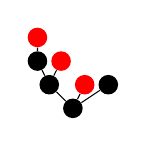
\begin{tikzpicture}[scale=.2]
\node[circle, scale=0.75, fill] (tid0) at (3,1.5){};
\node[circle, scale=0.75, fill] (tid1) at (1.5,3){};
\node[circle, scale=0.75, fill] (tid4) at (0.75,4.5){};
\node[circle, scale=0.75, fill, red] (tid6) at (0.75,6){};
\draw[](tid4) -- (tid6);
\node[circle, scale=0.75, fill, red] (tid5) at (2.25,4.5){};
\draw[](tid1) -- (tid4);
\draw[](tid1) -- (tid5);
\node[circle, scale=0.75, fill, red] (tid2) at (3.75,3){};
\node[circle, scale=0.75, fill] (tid3) at (5.25,3){};
\draw[](tid0) -- (tid1);
\draw[](tid0) -- (tid2);
\draw[](tid0) -- (tid3);
\end{tikzpicture}
\nodepart{three}
\footnotesize{4.47685}
\nodepart{four}
\footnotesize{$33\:33\:33$}
};
 & 
\node[draw=black, rectangle split,  rectangle split parts=4] (sn0x2512760){
\footnotesize{0.222222}
\nodepart{two}
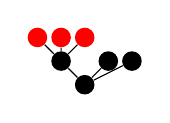
\begin{tikzpicture}[scale=.2]
\node[circle, scale=0.75, fill] (tid0) at (3.75,1.5){};
\node[circle, scale=0.75, fill] (tid1) at (2.25,3){};
\node[circle, scale=0.75, fill, red] (tid4) at (0.75,4.5){};
\node[circle, scale=0.75, fill, red] (tid5) at (2.25,4.5){};
\node[circle, scale=0.75, fill, red] (tid6) at (3.75,4.5){};
\draw[](tid1) -- (tid4);
\draw[](tid1) -- (tid5);
\draw[](tid1) -- (tid6);
\node[circle, scale=0.75, fill] (tid2) at (5.25,3){};
\node[circle, scale=0.75, fill] (tid3) at (6.75,3){};
\draw[](tid0) -- (tid1);
\draw[](tid0) -- (tid2);
\draw[](tid0) -- (tid3);
\end{tikzpicture}
\nodepart{three}
\footnotesize{4.18519}
\nodepart{four}
\footnotesize{$1$}
};
 & 
\node[draw=black, rectangle split,  rectangle split parts=4] (sn0x2511e20){
\footnotesize{0.0740741}
\nodepart{two}
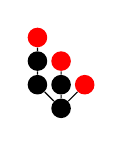
\begin{tikzpicture}[scale=.2]
\node[circle, scale=0.75, fill] (tid0) at (2.25,1.5){};
\node[circle, scale=0.75, fill] (tid1) at (0.75,3){};
\node[circle, scale=0.75, fill] (tid4) at (0.75,4.5){};
\node[circle, scale=0.75, fill, red] (tid6) at (0.75,6){};
\draw[](tid4) -- (tid6);
\draw[](tid1) -- (tid4);
\node[circle, scale=0.75, fill] (tid2) at (2.25,3){};
\node[circle, scale=0.75, fill, red] (tid5) at (2.25,4.5){};
\draw[](tid2) -- (tid5);
\node[circle, scale=0.75, fill, red] (tid3) at (3.75,3){};
\draw[](tid0) -- (tid1);
\draw[](tid0) -- (tid2);
\draw[](tid0) -- (tid3);
\end{tikzpicture}
\nodepart{three}
\footnotesize{4.5162}
\nodepart{four}
\footnotesize{$33\:33\:33$}
};
 & 
\node[draw=black, rectangle split,  rectangle split parts=4] (sn0x25132f0){
\footnotesize{0.222222}
\nodepart{two}
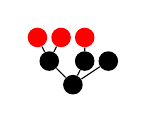
\begin{tikzpicture}[scale=.2]
\node[circle, scale=0.75, fill] (tid0) at (3,1.5){};
\node[circle, scale=0.75, fill] (tid1) at (1.5,3){};
\node[circle, scale=0.75, fill, red] (tid4) at (0.75,4.5){};
\node[circle, scale=0.75, fill, red] (tid5) at (2.25,4.5){};
\draw[](tid1) -- (tid4);
\draw[](tid1) -- (tid5);
\node[circle, scale=0.75, fill] (tid2) at (3.75,3){};
\node[circle, scale=0.75, fill, red] (tid6) at (3.75,4.5){};
\draw[](tid2) -- (tid6);
\node[circle, scale=0.75, fill] (tid3) at (5.25,3){};
\draw[](tid0) -- (tid1);
\draw[](tid0) -- (tid2);
\draw[](tid0) -- (tid3);
\end{tikzpicture}
\nodepart{three}
\footnotesize{4.2037}
\nodepart{four}
\footnotesize{$33\:67$}
};
 & 
\\
};
\end{scope}
\begin{scope}[yshift=\leveltopIIIII cm]
\matrix (line5) [column sep=1cm] {
\node[draw=black, rectangle split,  rectangle split parts=4] (sn0x250eda0){
\footnotesize{0.0123457}
\nodepart{two}
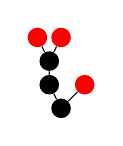
\begin{tikzpicture}[scale=.2]
\node[circle, scale=0.75, fill] (tid0) at (2.25,1.5){};
\node[circle, scale=0.75, fill] (tid1) at (1.5,3){};
\node[circle, scale=0.75, fill] (tid3) at (1.5,4.5){};
\node[circle, scale=0.75, fill, red] (tid4) at (0.75,6){};
\node[circle, scale=0.75, fill, red] (tid5) at (2.25,6){};
\draw[](tid3) -- (tid4);
\draw[](tid3) -- (tid5);
\draw[](tid1) -- (tid3);
\node[circle, scale=0.75, fill, red] (tid2) at (3.75,3){};
\draw[](tid0) -- (tid1);
\draw[](tid0) -- (tid2);
\end{tikzpicture}
\nodepart{three}
\footnotesize{4.58333}
\nodepart{four}
\footnotesize{$33\:67$}
};
 & 
\node[draw=black, rectangle split,  rectangle split parts=4] (sn0x250ea40){
\footnotesize{0.197531}
\nodepart{two}
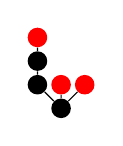
\begin{tikzpicture}[scale=.2]
\node[circle, scale=0.75, fill] (tid0) at (2.25,1.5){};
\node[circle, scale=0.75, fill] (tid1) at (0.75,3){};
\node[circle, scale=0.75, fill] (tid4) at (0.75,4.5){};
\node[circle, scale=0.75, fill, red] (tid5) at (0.75,6){};
\draw[](tid4) -- (tid5);
\draw[](tid1) -- (tid4);
\node[circle, scale=0.75, fill, red] (tid2) at (2.25,3){};
\node[circle, scale=0.75, fill, red] (tid3) at (3.75,3){};
\draw[](tid0) -- (tid1);
\draw[](tid0) -- (tid2);
\draw[](tid0) -- (tid3);
\end{tikzpicture}
\nodepart{three}
\footnotesize{4.23148}
\nodepart{four}
\footnotesize{$67\:33$}
};
 & 
\node[draw=black, rectangle split,  rectangle split parts=4] (sn0x2510810){
\footnotesize{0.148148}
\nodepart{two}
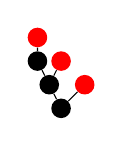
\begin{tikzpicture}[scale=.2]
\node[circle, scale=0.75, fill] (tid0) at (2.25,1.5){};
\node[circle, scale=0.75, fill] (tid1) at (1.5,3){};
\node[circle, scale=0.75, fill] (tid3) at (0.75,4.5){};
\node[circle, scale=0.75, fill, red] (tid5) at (0.75,6){};
\draw[](tid3) -- (tid5);
\node[circle, scale=0.75, fill, red] (tid4) at (2.25,4.5){};
\draw[](tid1) -- (tid3);
\draw[](tid1) -- (tid4);
\node[circle, scale=0.75, fill, red] (tid2) at (3.75,3){};
\draw[](tid0) -- (tid1);
\draw[](tid0) -- (tid2);
\end{tikzpicture}
\nodepart{three}
\footnotesize{4.34722}
\nodepart{four}
\footnotesize{$33\:33\:33$}
};
 & 
\node[draw=black, rectangle split,  rectangle split parts=4] (sn0x2511490){
\footnotesize{0.444444}
\nodepart{two}
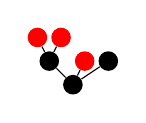
\begin{tikzpicture}[scale=.2]
\node[circle, scale=0.75, fill] (tid0) at (3,1.5){};
\node[circle, scale=0.75, fill] (tid1) at (1.5,3){};
\node[circle, scale=0.75, fill, red] (tid4) at (0.75,4.5){};
\node[circle, scale=0.75, fill, red] (tid5) at (2.25,4.5){};
\draw[](tid1) -- (tid4);
\draw[](tid1) -- (tid5);
\node[circle, scale=0.75, fill, red] (tid2) at (3.75,3){};
\node[circle, scale=0.75, fill] (tid3) at (5.25,3){};
\draw[](tid0) -- (tid1);
\draw[](tid0) -- (tid2);
\draw[](tid0) -- (tid3);
\end{tikzpicture}
\nodepart{three}
\footnotesize{3.85185}
\nodepart{four}
\footnotesize{$67\:33$}
};
 & 
\node[draw=black, rectangle split,  rectangle split parts=4] (sn0x2513e00){
\footnotesize{0.0246914}
\nodepart{two}
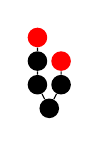
\begin{tikzpicture}[scale=.2]
\node[circle, scale=0.75, fill] (tid0) at (1.5,1.5){};
\node[circle, scale=0.75, fill] (tid1) at (0.75,3){};
\node[circle, scale=0.75, fill] (tid3) at (0.75,4.5){};
\node[circle, scale=0.75, fill, red] (tid5) at (0.75,6){};
\draw[](tid3) -- (tid5);
\draw[](tid1) -- (tid3);
\node[circle, scale=0.75, fill] (tid2) at (2.25,3){};
\node[circle, scale=0.75, fill, red] (tid4) at (2.25,4.5){};
\draw[](tid2) -- (tid4);
\draw[](tid0) -- (tid1);
\draw[](tid0) -- (tid2);
\end{tikzpicture}
\nodepart{three}
\footnotesize{4.4375}
\nodepart{four}
\footnotesize{$50\:50$}
};
 & 
\node[draw=black, rectangle split,  rectangle split parts=4] (sn0x2513810){
\footnotesize{0.17284}
\nodepart{two}
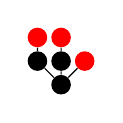
\begin{tikzpicture}[scale=.2]
\node[circle, scale=0.75, fill] (tid0) at (2.25,1.5){};
\node[circle, scale=0.75, fill] (tid1) at (0.75,3){};
\node[circle, scale=0.75, fill, red] (tid4) at (0.75,4.5){};
\draw[](tid1) -- (tid4);
\node[circle, scale=0.75, fill] (tid2) at (2.25,3){};
\node[circle, scale=0.75, fill, red] (tid5) at (2.25,4.5){};
\draw[](tid2) -- (tid5);
\node[circle, scale=0.75, fill, red] (tid3) at (3.75,3){};
\draw[](tid0) -- (tid1);
\draw[](tid0) -- (tid2);
\draw[](tid0) -- (tid3);
\end{tikzpicture}
\nodepart{three}
\footnotesize{3.87963}
\nodepart{four}
\footnotesize{$67\:33$}
};
 & 
\\
};
\end{scope}
\begin{scope}[yshift=\leveltopIIIIII cm]
\matrix (line6) [column sep=1cm] {
\node[draw=black, rectangle split,  rectangle split parts=4] (sn0x250f0b0){
\footnotesize{0.00411523}
\nodepart{two}
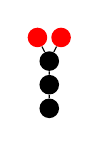
\begin{tikzpicture}[scale=.2]
\node[circle, scale=0.75, fill] (tid0) at (1.5,1.5){};
\node[circle, scale=0.75, fill] (tid1) at (1.5,3){};
\node[circle, scale=0.75, fill] (tid2) at (1.5,4.5){};
\node[circle, scale=0.75, fill, red] (tid3) at (0.75,6){};
\node[circle, scale=0.75, fill, red] (tid4) at (2.25,6){};
\draw[](tid2) -- (tid3);
\draw[](tid2) -- (tid4);
\draw[](tid1) -- (tid2);
\draw[](tid0) -- (tid1);
\end{tikzpicture}
\nodepart{three}
\footnotesize{4.5}
\nodepart{four}
\footnotesize{$1$}
};
 & 
\node[draw=black, rectangle split,  rectangle split parts=4] (sn0x250f180){
\footnotesize{0.201646}
\nodepart{two}
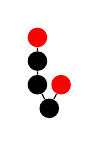
\begin{tikzpicture}[scale=.2]
\node[circle, scale=0.75, fill] (tid0) at (1.5,1.5){};
\node[circle, scale=0.75, fill] (tid1) at (0.75,3){};
\node[circle, scale=0.75, fill] (tid3) at (0.75,4.5){};
\node[circle, scale=0.75, fill, red] (tid4) at (0.75,6){};
\draw[](tid3) -- (tid4);
\draw[](tid1) -- (tid3);
\node[circle, scale=0.75, fill, red] (tid2) at (2.25,3){};
\draw[](tid0) -- (tid1);
\draw[](tid0) -- (tid2);
\end{tikzpicture}
\nodepart{three}
\footnotesize{4.125}
\nodepart{four}
\footnotesize{$50\:50$}
};
 & 
\node[draw=black, rectangle split,  rectangle split parts=4] (sn0x2510250){
\footnotesize{0.477366}
\nodepart{two}
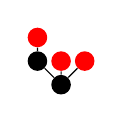
\begin{tikzpicture}[scale=.2]
\node[circle, scale=0.75, fill] (tid0) at (2.25,1.5){};
\node[circle, scale=0.75, fill] (tid1) at (0.75,3){};
\node[circle, scale=0.75, fill, red] (tid4) at (0.75,4.5){};
\draw[](tid1) -- (tid4);
\node[circle, scale=0.75, fill, red] (tid2) at (2.25,3){};
\node[circle, scale=0.75, fill, red] (tid3) at (3.75,3){};
\draw[](tid0) -- (tid1);
\draw[](tid0) -- (tid2);
\draw[](tid0) -- (tid3);
\end{tikzpicture}
\nodepart{three}
\footnotesize{3.44444}
\nodepart{four}
\footnotesize{$67\:33$}
};
 & 
\node[draw=black, rectangle split,  rectangle split parts=4] (sn0x2511820){
\footnotesize{0.0493827}
\nodepart{two}
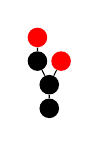
\begin{tikzpicture}[scale=.2]
\node[circle, scale=0.75, fill] (tid0) at (1.5,1.5){};
\node[circle, scale=0.75, fill] (tid1) at (1.5,3){};
\node[circle, scale=0.75, fill] (tid2) at (0.75,4.5){};
\node[circle, scale=0.75, fill, red] (tid4) at (0.75,6){};
\draw[](tid2) -- (tid4);
\node[circle, scale=0.75, fill, red] (tid3) at (2.25,4.5){};
\draw[](tid1) -- (tid2);
\draw[](tid1) -- (tid3);
\draw[](tid0) -- (tid1);
\end{tikzpicture}
\nodepart{three}
\footnotesize{4.25}
\nodepart{four}
\footnotesize{$50\:50$}
};
 & 
\node[draw=black, rectangle split,  rectangle split parts=4] (sn0x2510fd0){
\footnotesize{0.197531}
\nodepart{two}
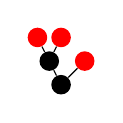
\begin{tikzpicture}[scale=.2]
\node[circle, scale=0.75, fill] (tid0) at (2.25,1.5){};
\node[circle, scale=0.75, fill] (tid1) at (1.5,3){};
\node[circle, scale=0.75, fill, red] (tid3) at (0.75,4.5){};
\node[circle, scale=0.75, fill, red] (tid4) at (2.25,4.5){};
\draw[](tid1) -- (tid3);
\draw[](tid1) -- (tid4);
\node[circle, scale=0.75, fill, red] (tid2) at (3.75,3){};
\draw[](tid0) -- (tid1);
\draw[](tid0) -- (tid2);
\end{tikzpicture}
\nodepart{three}
\footnotesize{3.66667}
\nodepart{four}
\footnotesize{$67\:33$}
};
 & 
\node[draw=black, rectangle split,  rectangle split parts=4] (sn0x2514110){
\footnotesize{0.0699589}
\nodepart{two}
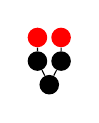
\begin{tikzpicture}[scale=.2]
\node[circle, scale=0.75, fill] (tid0) at (1.5,1.5){};
\node[circle, scale=0.75, fill] (tid1) at (0.75,3){};
\node[circle, scale=0.75, fill, red] (tid3) at (0.75,4.5){};
\draw[](tid1) -- (tid3);
\node[circle, scale=0.75, fill] (tid2) at (2.25,3){};
\node[circle, scale=0.75, fill, red] (tid4) at (2.25,4.5){};
\draw[](tid2) -- (tid4);
\draw[](tid0) -- (tid1);
\draw[](tid0) -- (tid2);
\end{tikzpicture}
\nodepart{three}
\footnotesize{3.75}
\nodepart{four}
\footnotesize{$1$}
};
 & 
\\
};
\end{scope}
\begin{scope}[yshift=\leveltopIIIIIII cm]
\matrix (line7) [column sep=1cm] {
\node[draw=black, rectangle split,  rectangle split parts=4] (sn0x250f520){
\footnotesize{0.12963}
\nodepart{two}
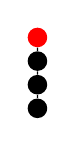
\begin{tikzpicture}[scale=.2]
\node[circle, scale=0.75, fill] (tid0) at (0.75,1.5){};
\node[circle, scale=0.75, fill] (tid1) at (0.75,3){};
\node[circle, scale=0.75, fill] (tid2) at (0.75,4.5){};
\node[circle, scale=0.75, fill, red] (tid3) at (0.75,6){};
\draw[](tid2) -- (tid3);
\draw[](tid1) -- (tid2);
\draw[](tid0) -- (tid1);
\end{tikzpicture}
\nodepart{three}
\footnotesize{4}
\nodepart{four}
\footnotesize{$1$}
};
 & 
\node[draw=black, rectangle split,  rectangle split parts=4] (sn0x250f860){
\footnotesize{0.620713}
\nodepart{two}
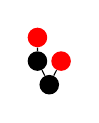
\begin{tikzpicture}[scale=.2]
\node[circle, scale=0.75, fill] (tid0) at (1.5,1.5){};
\node[circle, scale=0.75, fill] (tid1) at (0.75,3){};
\node[circle, scale=0.75, fill, red] (tid3) at (0.75,4.5){};
\draw[](tid1) -- (tid3);
\node[circle, scale=0.75, fill, red] (tid2) at (2.25,3){};
\draw[](tid0) -- (tid1);
\draw[](tid0) -- (tid2);
\end{tikzpicture}
\nodepart{three}
\footnotesize{3.25}
\nodepart{four}
\footnotesize{$50\:50$}
};
 & 
\node[draw=black, rectangle split,  rectangle split parts=4] (sn0x2510100){
\footnotesize{0.159122}
\nodepart{two}
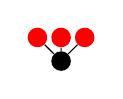
\begin{tikzpicture}[scale=.2]
\node[circle, scale=0.75, fill] (tid0) at (2.25,1.5){};
\node[circle, scale=0.75, fill, red] (tid1) at (0.75,3){};
\node[circle, scale=0.75, fill, red] (tid2) at (2.25,3){};
\node[circle, scale=0.75, fill, red] (tid3) at (3.75,3){};
\draw[](tid0) -- (tid1);
\draw[](tid0) -- (tid2);
\draw[](tid0) -- (tid3);
\end{tikzpicture}
\nodepart{three}
\footnotesize{2.83333}
\nodepart{four}
\footnotesize{$1$}
};
 & 
\node[draw=black, rectangle split,  rectangle split parts=4] (sn0x25110a0){
\footnotesize{0.090535}
\nodepart{two}
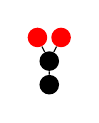
\begin{tikzpicture}[scale=.2]
\node[circle, scale=0.75, fill] (tid0) at (1.5,1.5){};
\node[circle, scale=0.75, fill] (tid1) at (1.5,3){};
\node[circle, scale=0.75, fill, red] (tid2) at (0.75,4.5){};
\node[circle, scale=0.75, fill, red] (tid3) at (2.25,4.5){};
\draw[](tid1) -- (tid2);
\draw[](tid1) -- (tid3);
\draw[](tid0) -- (tid1);
\end{tikzpicture}
\nodepart{three}
\footnotesize{3.5}
\nodepart{four}
\footnotesize{$1$}
};
 & 
\\
};
\end{scope}
\begin{scope}[yshift=\leveltopIIIIIIII cm]
\matrix (line8) [column sep=1cm] {
\node[draw=black, rectangle split,  rectangle split parts=4] (sn0x250f5f0){
\footnotesize{0.530521}
\nodepart{two}
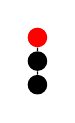
\begin{tikzpicture}[scale=.2]
\node[circle, scale=0.75, fill] (tid0) at (0.75,1.5){};
\node[circle, scale=0.75, fill] (tid1) at (0.75,3){};
\node[circle, scale=0.75, fill, red] (tid2) at (0.75,4.5){};
\draw[](tid1) -- (tid2);
\draw[](tid0) -- (tid1);
\end{tikzpicture}
\nodepart{three}
\footnotesize{3}
\nodepart{four}
\footnotesize{$1$}
};
 & 
\node[draw=black, rectangle split,  rectangle split parts=4] (sn0x250fe10){
\footnotesize{0.469479}
\nodepart{two}

\begin{tikzpicture}[scale=.2]
\node[circle, scale=0.75, fill] (tid0) at (1.5,1.5){};
\node[circle, scale=0.75, fill, red] (tid1) at (0.75,3){};
\node[circle, scale=0.75, fill, red] (tid2) at (2.25,3){};
\draw[](tid0) -- (tid1);
\draw[](tid0) -- (tid2);
\end{tikzpicture}
\nodepart{three}
\footnotesize{2.5}
\nodepart{four}
\footnotesize{$1$}
};
 & 
\\
};
\end{scope}
\begin{scope}[yshift=\leveltopIIIIIIIII cm]
\matrix (line9) [column sep=1cm] {
\node[draw=black, rectangle split,  rectangle split parts=4] (sn0x250f3d0){
\footnotesize{1}
\nodepart{two}

\begin{tikzpicture}[scale=.2]
\node[circle, scale=0.75, fill] (tid0) at (0.75,1.5){};
\node[circle, scale=0.75, fill, red] (tid1) at (0.75,3){};
\draw[](tid0) -- (tid1);
\end{tikzpicture}
\nodepart{three}
\footnotesize{2}
\nodepart{four}
\footnotesize{$1$}
};
 & 
\\
};
\end{scope}
\begin{scope}[yshift=\leveltopIIIIIIIIII cm]
\matrix (line10) [column sep=1cm] {
\node[draw=black, rectangle split,  rectangle split parts=4] (sn0x250e760){
\footnotesize{1}
\nodepart{two}

\begin{tikzpicture}[scale=.2]
\node[circle, scale=0.75, fill, red] (tid0) at (0.75,1.5){};
\end{tikzpicture}
\nodepart{three}
\footnotesize{1}
\nodepart{four}
\footnotesize{$$}
};
 & 
\\
};
\end{scope}
\begin{scope}[yshift=\leveltopIIIIIIIIIII cm]
\matrix (line11) [column sep=1cm] {
\\
};
\end{scope}
\draw (sn0x250ba90.south) -- (sn0x250d5a0.north);
\draw (sn0x250ba90.south) -- (sn0x250c380.north);
\draw (sn0x250d5a0.south) -- (sn0x250de90.north);
\draw (sn0x250d5a0.south) -- (sn0x250d150.north);
\draw (sn0x250c380.south) -- (sn0x2512830.north);
\draw (sn0x250c380.south) -- (sn0x250d150.north);
\draw (sn0x250c380.south) -- (sn0x2512ab0.north);
\draw (sn0x250de90.south) -- (sn0x250dd40.north);
\draw (sn0x250de90.south) -- (sn0x250e690.north);
\draw (sn0x250d150.south) -- (sn0x250e690.north);
\draw (sn0x250d150.south) -- (sn0x2512760.north);
\draw (sn0x2512830.south) -- (sn0x2511e20.north);
\draw (sn0x2512830.south) -- (sn0x250e690.north);
\draw (sn0x2512830.south) -- (sn0x25132f0.north);
\draw (sn0x2512ab0.south) -- (sn0x25132f0.north);
\draw (sn0x2512ab0.south) -- (sn0x2512760.north);
\draw (sn0x250dd40.south) -- (sn0x250eda0.north);
\draw (sn0x250dd40.south) -- (sn0x250ea40.north);
\draw (sn0x250e690.south) -- (sn0x2510810.north);
\draw (sn0x250e690.south) -- (sn0x250ea40.north);
\draw (sn0x250e690.south) -- (sn0x2511490.north);
\draw (sn0x2512760.south) -- (sn0x2511490.north);
\draw (sn0x2511e20.south) -- (sn0x2513e00.north);
\draw (sn0x2511e20.south) -- (sn0x250ea40.north);
\draw (sn0x2511e20.south) -- (sn0x2513810.north);
\draw (sn0x25132f0.south) -- (sn0x2513810.north);
\draw (sn0x25132f0.south) -- (sn0x2511490.north);
\draw (sn0x250eda0.south) -- (sn0x250f0b0.north);
\draw (sn0x250eda0.south) -- (sn0x250f180.north);
\draw (sn0x250ea40.south) -- (sn0x250f180.north);
\draw (sn0x250ea40.south) -- (sn0x2510250.north);
\draw (sn0x2510810.south) -- (sn0x2511820.north);
\draw (sn0x2510810.south) -- (sn0x250f180.north);
\draw (sn0x2510810.south) -- (sn0x2510fd0.north);
\draw (sn0x2511490.south) -- (sn0x2510fd0.north);
\draw (sn0x2511490.south) -- (sn0x2510250.north);
\draw (sn0x2513e00.south) -- (sn0x250f180.north);
\draw (sn0x2513e00.south) -- (sn0x2514110.north);
\draw (sn0x2513810.south) -- (sn0x2514110.north);
\draw (sn0x2513810.south) -- (sn0x2510250.north);
\draw (sn0x250f0b0.south) -- (sn0x250f520.north);
\draw (sn0x250f180.south) -- (sn0x250f520.north);
\draw (sn0x250f180.south) -- (sn0x250f860.north);
\draw (sn0x2510250.south) -- (sn0x250f860.north);
\draw (sn0x2510250.south) -- (sn0x2510100.north);
\draw (sn0x2511820.south) -- (sn0x250f520.north);
\draw (sn0x2511820.south) -- (sn0x25110a0.north);
\draw (sn0x2510fd0.south) -- (sn0x25110a0.north);
\draw (sn0x2510fd0.south) -- (sn0x250f860.north);
\draw (sn0x2514110.south) -- (sn0x250f860.north);
\draw (sn0x250f520.south) -- (sn0x250f5f0.north);
\draw (sn0x250f860.south) -- (sn0x250f5f0.north);
\draw (sn0x250f860.south) -- (sn0x250fe10.north);
\draw (sn0x2510100.south) -- (sn0x250fe10.north);
\draw (sn0x25110a0.south) -- (sn0x250f5f0.north);
\draw (sn0x250f5f0.south) -- (sn0x250f3d0.north);
\draw (sn0x250fe10.south) -- (sn0x250f3d0.north);
\draw (sn0x250f3d0.south) -- (sn0x250e760.north);
\end{tikzpicture}

%%% Local Variables:
%%% TeX-master: "thesis/thesis.tex"
%%% End: 
\renewcommand{\leveltopI}{-15cm + \leveltop}
\renewcommand{\leveltopII}{-15cm + \leveltopI}
\renewcommand{\leveltopIII}{-15cm + \leveltopII}
\renewcommand{\leveltopIIII}{-15cm + \leveltopIII}
\renewcommand{\leveltopIIIII}{-15cm + \leveltopIIII}
\renewcommand{\leveltopIIIIII}{-15cm + \leveltopIIIII}
\renewcommand{\leveltopIIIIIII}{-15cm + \leveltopIIIIII}
\renewcommand{\leveltopIIIIIIII}{-15cm + \leveltopIIIIIII}
\renewcommand{\leveltopIIIIIIIII}{-15cm + \leveltopIIIIIIII}
\renewcommand{\leveltopIIIIIIIIII}{-15cm + \leveltopIIIIIIIII}
\begin{tikzpicture}[scale=.2, anchor=south]
\begin{scope}[yshift=\leveltopI cm]
\matrix (line1) [column sep=1cm] {
\node[draw=black, rectangle split,  rectangle split parts=4] (sn0x250cfd0){
\footnotesize{1}
\nodepart{two}
\begin{tikzpicture}[scale=.2]
\node[circle, scale=0.75, fill] (tid0) at (4.5,1.5){};
\node[circle, scale=0.75, fill] (tid1) at (3,3){};
\node[circle, scale=0.75, fill] (tid4) at (1.5,4.5){};
\node[circle, scale=0.75, fill, red] (tid8) at (0.75,6){};
\node[circle, scale=0.75, fill, red] (tid9) at (2.25,6){};
\draw[](tid4) -- (tid8);
\draw[](tid4) -- (tid9);
\node[circle, scale=0.75, fill, red] (tid5) at (3.75,4.5){};
\node[circle, scale=0.75, fill] (tid6) at (5.25,4.5){};
\draw[](tid1) -- (tid4);
\draw[](tid1) -- (tid5);
\draw[](tid1) -- (tid6);
\node[circle, scale=0.75, fill] (tid2) at (6.75,3){};
\node[circle, scale=0.75, fill] (tid7) at (6.75,4.5){};
\draw[](tid2) -- (tid7);
\node[circle, scale=0.75, fill] (tid3) at (8.25,3){};
\draw[](tid0) -- (tid1);
\draw[](tid0) -- (tid2);
\draw[](tid0) -- (tid3);
\end{tikzpicture}
\nodepart{three}
\footnotesize{5.37009}
\nodepart{four}
\footnotesize{$17\:17\:33\:33$}
};
 & 
\\
};
\end{scope}
\begin{scope}[yshift=\leveltopII cm]
\matrix (line2) [column sep=1cm] {
\node[draw=black, rectangle split,  rectangle split parts=4] (sn0x25141e0){
\footnotesize{0.166667}
\nodepart{two}
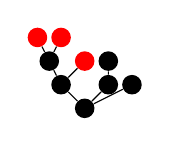
\begin{tikzpicture}[scale=.2]
\node[circle, scale=0.75, fill] (tid0) at (3.75,1.5){};
\node[circle, scale=0.75, fill] (tid1) at (2.25,3){};
\node[circle, scale=0.75, fill] (tid4) at (1.5,4.5){};
\node[circle, scale=0.75, fill, red] (tid7) at (0.75,6){};
\node[circle, scale=0.75, fill, red] (tid8) at (2.25,6){};
\draw[](tid4) -- (tid7);
\draw[](tid4) -- (tid8);
\node[circle, scale=0.75, fill, red] (tid5) at (3.75,4.5){};
\draw[](tid1) -- (tid4);
\draw[](tid1) -- (tid5);
\node[circle, scale=0.75, fill] (tid2) at (5.25,3){};
\node[circle, scale=0.75, fill] (tid6) at (5.25,4.5){};
\draw[](tid2) -- (tid6);
\node[circle, scale=0.75, fill] (tid3) at (6.75,3){};
\draw[](tid0) -- (tid1);
\draw[](tid0) -- (tid2);
\draw[](tid0) -- (tid3);
\end{tikzpicture}
\nodepart{three}
\footnotesize{5.12311}
\nodepart{four}
\footnotesize{$33\:67$}
};
 & 
\node[draw=black, rectangle split,  rectangle split parts=4] (sn0x2514f90){
\footnotesize{0.166667}
\nodepart{two}
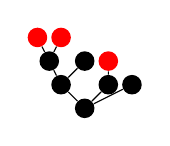
\begin{tikzpicture}[scale=.2]
\node[circle, scale=0.75, fill] (tid0) at (3.75,1.5){};
\node[circle, scale=0.75, fill] (tid1) at (2.25,3){};
\node[circle, scale=0.75, fill] (tid4) at (1.5,4.5){};
\node[circle, scale=0.75, fill, red] (tid7) at (0.75,6){};
\node[circle, scale=0.75, fill, red] (tid8) at (2.25,6){};
\draw[](tid4) -- (tid7);
\draw[](tid4) -- (tid8);
\node[circle, scale=0.75, fill] (tid5) at (3.75,4.5){};
\draw[](tid1) -- (tid4);
\draw[](tid1) -- (tid5);
\node[circle, scale=0.75, fill] (tid2) at (5.25,3){};
\node[circle, scale=0.75, fill, red] (tid6) at (5.25,4.5){};
\draw[](tid2) -- (tid6);
\node[circle, scale=0.75, fill] (tid3) at (6.75,3){};
\draw[](tid0) -- (tid1);
\draw[](tid0) -- (tid2);
\draw[](tid0) -- (tid3);
\end{tikzpicture}
\nodepart{three}
\footnotesize{5.11437}
\nodepart{four}
\footnotesize{$67\:33$}
};
 & 
\node[draw=black, rectangle split,  rectangle split parts=4] (sn0x2514650){
\footnotesize{0.333333}
\nodepart{two}
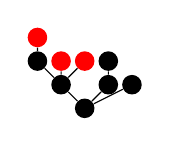
\begin{tikzpicture}[scale=.2]
\node[circle, scale=0.75, fill] (tid0) at (3.75,1.5){};
\node[circle, scale=0.75, fill] (tid1) at (2.25,3){};
\node[circle, scale=0.75, fill] (tid4) at (0.75,4.5){};
\node[circle, scale=0.75, fill, red] (tid8) at (0.75,6){};
\draw[](tid4) -- (tid8);
\node[circle, scale=0.75, fill, red] (tid5) at (2.25,4.5){};
\node[circle, scale=0.75, fill, red] (tid6) at (3.75,4.5){};
\draw[](tid1) -- (tid4);
\draw[](tid1) -- (tid5);
\draw[](tid1) -- (tid6);
\node[circle, scale=0.75, fill] (tid2) at (5.25,3){};
\node[circle, scale=0.75, fill] (tid7) at (5.25,4.5){};
\draw[](tid2) -- (tid7);
\node[circle, scale=0.75, fill] (tid3) at (6.75,3){};
\draw[](tid0) -- (tid1);
\draw[](tid0) -- (tid2);
\draw[](tid0) -- (tid3);
\end{tikzpicture}
\nodepart{three}
\footnotesize{4.99949}
\nodepart{four}
\footnotesize{$67\:17\:17$}
};
 & 
\node[draw=black, rectangle split,  rectangle split parts=4] (sn0x250c380){
\footnotesize{0.333333}
\nodepart{two}
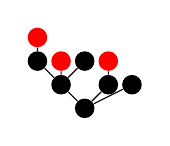
\begin{tikzpicture}[scale=.2]
\node[circle, scale=0.75, fill] (tid0) at (3.75,1.5){};
\node[circle, scale=0.75, fill] (tid1) at (2.25,3){};
\node[circle, scale=0.75, fill] (tid4) at (0.75,4.5){};
\node[circle, scale=0.75, fill, red] (tid8) at (0.75,6){};
\draw[](tid4) -- (tid8);
\node[circle, scale=0.75, fill, red] (tid5) at (2.25,4.5){};
\node[circle, scale=0.75, fill] (tid6) at (3.75,4.5){};
\draw[](tid1) -- (tid4);
\draw[](tid1) -- (tid5);
\draw[](tid1) -- (tid6);
\node[circle, scale=0.75, fill] (tid2) at (5.25,3){};
\node[circle, scale=0.75, fill, red] (tid7) at (5.25,4.5){};
\draw[](tid2) -- (tid7);
\node[circle, scale=0.75, fill] (tid3) at (6.75,3){};
\draw[](tid0) -- (tid1);
\draw[](tid0) -- (tid2);
\draw[](tid0) -- (tid3);
\end{tikzpicture}
\nodepart{three}
\footnotesize{4.99203}
\nodepart{four}
\footnotesize{$33\:33\:33$}
};
 & 
\\
};
\end{scope}
\begin{scope}[yshift=\leveltopIII cm]
\matrix (line3) [column sep=1cm] {
\node[draw=black, rectangle split,  rectangle split parts=4] (sn0x25159a0){
\footnotesize{0.0555556}
\nodepart{two}
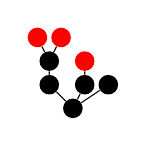
\begin{tikzpicture}[scale=.2]
\node[circle, scale=0.75, fill] (tid0) at (3,1.5){};
\node[circle, scale=0.75, fill] (tid1) at (1.5,3){};
\node[circle, scale=0.75, fill] (tid4) at (1.5,4.5){};
\node[circle, scale=0.75, fill, red] (tid6) at (0.75,6){};
\node[circle, scale=0.75, fill, red] (tid7) at (2.25,6){};
\draw[](tid4) -- (tid6);
\draw[](tid4) -- (tid7);
\draw[](tid1) -- (tid4);
\node[circle, scale=0.75, fill] (tid2) at (3.75,3){};
\node[circle, scale=0.75, fill, red] (tid5) at (3.75,4.5){};
\draw[](tid2) -- (tid5);
\node[circle, scale=0.75, fill] (tid3) at (5.25,3){};
\draw[](tid0) -- (tid1);
\draw[](tid0) -- (tid2);
\draw[](tid0) -- (tid3);
\end{tikzpicture}
\nodepart{three}
\footnotesize{4.90484}
\nodepart{four}
\footnotesize{$33\:67$}
};
 & 
\node[draw=black, rectangle split,  rectangle split parts=4] (sn0x2512830){
\footnotesize{0.555556}
\nodepart{two}
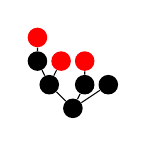
\begin{tikzpicture}[scale=.2]
\node[circle, scale=0.75, fill] (tid0) at (3,1.5){};
\node[circle, scale=0.75, fill] (tid1) at (1.5,3){};
\node[circle, scale=0.75, fill] (tid4) at (0.75,4.5){};
\node[circle, scale=0.75, fill, red] (tid7) at (0.75,6){};
\draw[](tid4) -- (tid7);
\node[circle, scale=0.75, fill, red] (tid5) at (2.25,4.5){};
\draw[](tid1) -- (tid4);
\draw[](tid1) -- (tid5);
\node[circle, scale=0.75, fill] (tid2) at (3.75,3){};
\node[circle, scale=0.75, fill, red] (tid6) at (3.75,4.5){};
\draw[](tid2) -- (tid6);
\node[circle, scale=0.75, fill] (tid3) at (5.25,3){};
\draw[](tid0) -- (tid1);
\draw[](tid0) -- (tid2);
\draw[](tid0) -- (tid3);
\end{tikzpicture}
\nodepart{three}
\footnotesize{4.73225}
\nodepart{four}
\footnotesize{$33\:33\:33$}
};
 & 
\node[draw=black, rectangle split,  rectangle split parts=4] (sn0x250de90){
\footnotesize{0.0555556}
\nodepart{two}
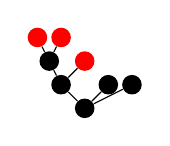
\begin{tikzpicture}[scale=.2]
\node[circle, scale=0.75, fill] (tid0) at (3.75,1.5){};
\node[circle, scale=0.75, fill] (tid1) at (2.25,3){};
\node[circle, scale=0.75, fill] (tid4) at (1.5,4.5){};
\node[circle, scale=0.75, fill, red] (tid6) at (0.75,6){};
\node[circle, scale=0.75, fill, red] (tid7) at (2.25,6){};
\draw[](tid4) -- (tid6);
\draw[](tid4) -- (tid7);
\node[circle, scale=0.75, fill, red] (tid5) at (3.75,4.5){};
\draw[](tid1) -- (tid4);
\draw[](tid1) -- (tid5);
\node[circle, scale=0.75, fill] (tid2) at (5.25,3){};
\node[circle, scale=0.75, fill] (tid3) at (6.75,3){};
\draw[](tid0) -- (tid1);
\draw[](tid0) -- (tid2);
\draw[](tid0) -- (tid3);
\end{tikzpicture}
\nodepart{three}
\footnotesize{4.8786}
\nodepart{four}
\footnotesize{$33\:67$}
};
 & 
\node[draw=black, rectangle split,  rectangle split parts=4] (sn0x2515ae0){
\footnotesize{0.0555556}
\nodepart{two}
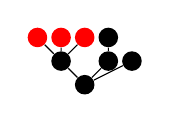
\begin{tikzpicture}[scale=.2]
\node[circle, scale=0.75, fill] (tid0) at (3.75,1.5){};
\node[circle, scale=0.75, fill] (tid1) at (2.25,3){};
\node[circle, scale=0.75, fill, red] (tid4) at (0.75,4.5){};
\node[circle, scale=0.75, fill, red] (tid5) at (2.25,4.5){};
\node[circle, scale=0.75, fill, red] (tid6) at (3.75,4.5){};
\draw[](tid1) -- (tid4);
\draw[](tid1) -- (tid5);
\draw[](tid1) -- (tid6);
\node[circle, scale=0.75, fill] (tid2) at (5.25,3){};
\node[circle, scale=0.75, fill] (tid7) at (5.25,4.5){};
\draw[](tid2) -- (tid7);
\node[circle, scale=0.75, fill] (tid3) at (6.75,3){};
\draw[](tid0) -- (tid1);
\draw[](tid0) -- (tid2);
\draw[](tid0) -- (tid3);
\end{tikzpicture}
\nodepart{three}
\footnotesize{4.53704}
\nodepart{four}
\footnotesize{$1$}
};
 & 
\node[draw=black, rectangle split,  rectangle split parts=4] (sn0x2512ab0){
\footnotesize{0.166667}
\nodepart{two}
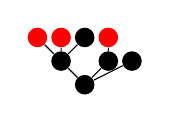
\begin{tikzpicture}[scale=.2]
\node[circle, scale=0.75, fill] (tid0) at (3.75,1.5){};
\node[circle, scale=0.75, fill] (tid1) at (2.25,3){};
\node[circle, scale=0.75, fill, red] (tid4) at (0.75,4.5){};
\node[circle, scale=0.75, fill, red] (tid5) at (2.25,4.5){};
\node[circle, scale=0.75, fill] (tid6) at (3.75,4.5){};
\draw[](tid1) -- (tid4);
\draw[](tid1) -- (tid5);
\draw[](tid1) -- (tid6);
\node[circle, scale=0.75, fill] (tid2) at (5.25,3){};
\node[circle, scale=0.75, fill, red] (tid7) at (5.25,4.5){};
\draw[](tid2) -- (tid7);
\node[circle, scale=0.75, fill] (tid3) at (6.75,3){};
\draw[](tid0) -- (tid1);
\draw[](tid0) -- (tid2);
\draw[](tid0) -- (tid3);
\end{tikzpicture}
\nodepart{three}
\footnotesize{4.53086}
\nodepart{four}
\footnotesize{$67\:33$}
};
 & 
\node[draw=black, rectangle split,  rectangle split parts=4] (sn0x250d150){
\footnotesize{0.111111}
\nodepart{two}
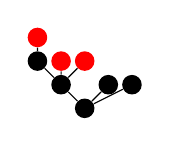
\begin{tikzpicture}[scale=.2]
\node[circle, scale=0.75, fill] (tid0) at (3.75,1.5){};
\node[circle, scale=0.75, fill] (tid1) at (2.25,3){};
\node[circle, scale=0.75, fill] (tid4) at (0.75,4.5){};
\node[circle, scale=0.75, fill, red] (tid7) at (0.75,6){};
\draw[](tid4) -- (tid7);
\node[circle, scale=0.75, fill, red] (tid5) at (2.25,4.5){};
\node[circle, scale=0.75, fill, red] (tid6) at (3.75,4.5){};
\draw[](tid1) -- (tid4);
\draw[](tid1) -- (tid5);
\draw[](tid1) -- (tid6);
\node[circle, scale=0.75, fill] (tid2) at (5.25,3){};
\node[circle, scale=0.75, fill] (tid3) at (6.75,3){};
\draw[](tid0) -- (tid1);
\draw[](tid0) -- (tid2);
\draw[](tid0) -- (tid3);
\end{tikzpicture}
\nodepart{three}
\footnotesize{4.71296}
\nodepart{four}
\footnotesize{$67\:33$}
};
 & 
\\
};
\end{scope}
\begin{scope}[yshift=\leveltopIIII cm]
\matrix (line4) [column sep=1cm] {
\node[draw=black, rectangle split,  rectangle split parts=4] (sn0x250dd40){
\footnotesize{0.037037}
\nodepart{two}
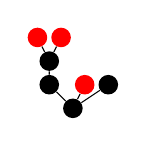
\begin{tikzpicture}[scale=.2]
\node[circle, scale=0.75, fill] (tid0) at (3,1.5){};
\node[circle, scale=0.75, fill] (tid1) at (1.5,3){};
\node[circle, scale=0.75, fill] (tid4) at (1.5,4.5){};
\node[circle, scale=0.75, fill, red] (tid5) at (0.75,6){};
\node[circle, scale=0.75, fill, red] (tid6) at (2.25,6){};
\draw[](tid4) -- (tid5);
\draw[](tid4) -- (tid6);
\draw[](tid1) -- (tid4);
\node[circle, scale=0.75, fill, red] (tid2) at (3.75,3){};
\node[circle, scale=0.75, fill] (tid3) at (5.25,3){};
\draw[](tid0) -- (tid1);
\draw[](tid0) -- (tid2);
\draw[](tid0) -- (tid3);
\end{tikzpicture}
\nodepart{three}
\footnotesize{4.6821}
\nodepart{four}
\footnotesize{$33\:67$}
};
 & 
\node[draw=black, rectangle split,  rectangle split parts=4] (sn0x2511e20){
\footnotesize{0.222222}
\nodepart{two}
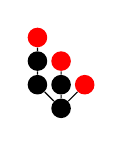
\begin{tikzpicture}[scale=.2]
\node[circle, scale=0.75, fill] (tid0) at (2.25,1.5){};
\node[circle, scale=0.75, fill] (tid1) at (0.75,3){};
\node[circle, scale=0.75, fill] (tid4) at (0.75,4.5){};
\node[circle, scale=0.75, fill, red] (tid6) at (0.75,6){};
\draw[](tid4) -- (tid6);
\draw[](tid1) -- (tid4);
\node[circle, scale=0.75, fill] (tid2) at (2.25,3){};
\node[circle, scale=0.75, fill, red] (tid5) at (2.25,4.5){};
\draw[](tid2) -- (tid5);
\node[circle, scale=0.75, fill, red] (tid3) at (3.75,3){};
\draw[](tid0) -- (tid1);
\draw[](tid0) -- (tid2);
\draw[](tid0) -- (tid3);
\end{tikzpicture}
\nodepart{three}
\footnotesize{4.5162}
\nodepart{four}
\footnotesize{$33\:33\:33$}
};
 & 
\node[draw=black, rectangle split,  rectangle split parts=4] (sn0x250e690){
\footnotesize{0.296296}
\nodepart{two}
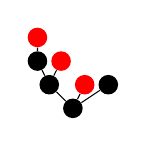
\begin{tikzpicture}[scale=.2]
\node[circle, scale=0.75, fill] (tid0) at (3,1.5){};
\node[circle, scale=0.75, fill] (tid1) at (1.5,3){};
\node[circle, scale=0.75, fill] (tid4) at (0.75,4.5){};
\node[circle, scale=0.75, fill, red] (tid6) at (0.75,6){};
\draw[](tid4) -- (tid6);
\node[circle, scale=0.75, fill, red] (tid5) at (2.25,4.5){};
\draw[](tid1) -- (tid4);
\draw[](tid1) -- (tid5);
\node[circle, scale=0.75, fill, red] (tid2) at (3.75,3){};
\node[circle, scale=0.75, fill] (tid3) at (5.25,3){};
\draw[](tid0) -- (tid1);
\draw[](tid0) -- (tid2);
\draw[](tid0) -- (tid3);
\end{tikzpicture}
\nodepart{three}
\footnotesize{4.47685}
\nodepart{four}
\footnotesize{$33\:33\:33$}
};
 & 
\node[draw=black, rectangle split,  rectangle split parts=4] (sn0x25132f0){
\footnotesize{0.351852}
\nodepart{two}
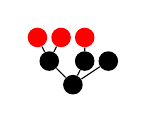
\begin{tikzpicture}[scale=.2]
\node[circle, scale=0.75, fill] (tid0) at (3,1.5){};
\node[circle, scale=0.75, fill] (tid1) at (1.5,3){};
\node[circle, scale=0.75, fill, red] (tid4) at (0.75,4.5){};
\node[circle, scale=0.75, fill, red] (tid5) at (2.25,4.5){};
\draw[](tid1) -- (tid4);
\draw[](tid1) -- (tid5);
\node[circle, scale=0.75, fill] (tid2) at (3.75,3){};
\node[circle, scale=0.75, fill, red] (tid6) at (3.75,4.5){};
\draw[](tid2) -- (tid6);
\node[circle, scale=0.75, fill] (tid3) at (5.25,3){};
\draw[](tid0) -- (tid1);
\draw[](tid0) -- (tid2);
\draw[](tid0) -- (tid3);
\end{tikzpicture}
\nodepart{three}
\footnotesize{4.2037}
\nodepart{four}
\footnotesize{$67\:33$}
};
 & 
\node[draw=black, rectangle split,  rectangle split parts=4] (sn0x2512760){
\footnotesize{0.0925926}
\nodepart{two}
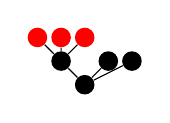
\begin{tikzpicture}[scale=.2]
\node[circle, scale=0.75, fill] (tid0) at (3.75,1.5){};
\node[circle, scale=0.75, fill] (tid1) at (2.25,3){};
\node[circle, scale=0.75, fill, red] (tid4) at (0.75,4.5){};
\node[circle, scale=0.75, fill, red] (tid5) at (2.25,4.5){};
\node[circle, scale=0.75, fill, red] (tid6) at (3.75,4.5){};
\draw[](tid1) -- (tid4);
\draw[](tid1) -- (tid5);
\draw[](tid1) -- (tid6);
\node[circle, scale=0.75, fill] (tid2) at (5.25,3){};
\node[circle, scale=0.75, fill] (tid3) at (6.75,3){};
\draw[](tid0) -- (tid1);
\draw[](tid0) -- (tid2);
\draw[](tid0) -- (tid3);
\end{tikzpicture}
\nodepart{three}
\footnotesize{4.18519}
\nodepart{four}
\footnotesize{$1$}
};
 & 
\\
};
\end{scope}
\begin{scope}[yshift=\leveltopIIIII cm]
\matrix (line5) [column sep=1cm] {
\node[draw=black, rectangle split,  rectangle split parts=4] (sn0x250eda0){
\footnotesize{0.0123457}
\nodepart{two}
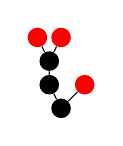
\begin{tikzpicture}[scale=.2]
\node[circle, scale=0.75, fill] (tid0) at (2.25,1.5){};
\node[circle, scale=0.75, fill] (tid1) at (1.5,3){};
\node[circle, scale=0.75, fill] (tid3) at (1.5,4.5){};
\node[circle, scale=0.75, fill, red] (tid4) at (0.75,6){};
\node[circle, scale=0.75, fill, red] (tid5) at (2.25,6){};
\draw[](tid3) -- (tid4);
\draw[](tid3) -- (tid5);
\draw[](tid1) -- (tid3);
\node[circle, scale=0.75, fill, red] (tid2) at (3.75,3){};
\draw[](tid0) -- (tid1);
\draw[](tid0) -- (tid2);
\end{tikzpicture}
\nodepart{three}
\footnotesize{4.58333}
\nodepart{four}
\footnotesize{$33\:67$}
};
 & 
\node[draw=black, rectangle split,  rectangle split parts=4] (sn0x250ea40){
\footnotesize{0.197531}
\nodepart{two}
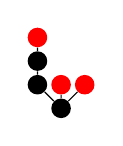
\begin{tikzpicture}[scale=.2]
\node[circle, scale=0.75, fill] (tid0) at (2.25,1.5){};
\node[circle, scale=0.75, fill] (tid1) at (0.75,3){};
\node[circle, scale=0.75, fill] (tid4) at (0.75,4.5){};
\node[circle, scale=0.75, fill, red] (tid5) at (0.75,6){};
\draw[](tid4) -- (tid5);
\draw[](tid1) -- (tid4);
\node[circle, scale=0.75, fill, red] (tid2) at (2.25,3){};
\node[circle, scale=0.75, fill, red] (tid3) at (3.75,3){};
\draw[](tid0) -- (tid1);
\draw[](tid0) -- (tid2);
\draw[](tid0) -- (tid3);
\end{tikzpicture}
\nodepart{three}
\footnotesize{4.23148}
\nodepart{four}
\footnotesize{$67\:33$}
};
 & 
\node[draw=black, rectangle split,  rectangle split parts=4] (sn0x2513e00){
\footnotesize{0.0740741}
\nodepart{two}
\begin{tikzpicture}[scale=.2]
\node[circle, scale=0.75, fill] (tid0) at (1.5,1.5){};
\node[circle, scale=0.75, fill] (tid1) at (0.75,3){};
\node[circle, scale=0.75, fill] (tid3) at (0.75,4.5){};
\node[circle, scale=0.75, fill, red] (tid5) at (0.75,6){};
\draw[](tid3) -- (tid5);
\draw[](tid1) -- (tid3);
\node[circle, scale=0.75, fill] (tid2) at (2.25,3){};
\node[circle, scale=0.75, fill, red] (tid4) at (2.25,4.5){};
\draw[](tid2) -- (tid4);
\draw[](tid0) -- (tid1);
\draw[](tid0) -- (tid2);
\end{tikzpicture}
\nodepart{three}
\footnotesize{4.4375}
\nodepart{four}
\footnotesize{$50\:50$}
};
 & 
\node[draw=black, rectangle split,  rectangle split parts=4] (sn0x2513810){
\footnotesize{0.308642}
\nodepart{two}
\begin{tikzpicture}[scale=.2]
\node[circle, scale=0.75, fill] (tid0) at (2.25,1.5){};
\node[circle, scale=0.75, fill] (tid1) at (0.75,3){};
\node[circle, scale=0.75, fill, red] (tid4) at (0.75,4.5){};
\draw[](tid1) -- (tid4);
\node[circle, scale=0.75, fill] (tid2) at (2.25,3){};
\node[circle, scale=0.75, fill, red] (tid5) at (2.25,4.5){};
\draw[](tid2) -- (tid5);
\node[circle, scale=0.75, fill, red] (tid3) at (3.75,3){};
\draw[](tid0) -- (tid1);
\draw[](tid0) -- (tid2);
\draw[](tid0) -- (tid3);
\end{tikzpicture}
\nodepart{three}
\footnotesize{3.87963}
\nodepart{four}
\footnotesize{$67\:33$}
};
 & 
\node[draw=black, rectangle split,  rectangle split parts=4] (sn0x2510810){
\footnotesize{0.0987654}
\nodepart{two}
\begin{tikzpicture}[scale=.2]
\node[circle, scale=0.75, fill] (tid0) at (2.25,1.5){};
\node[circle, scale=0.75, fill] (tid1) at (1.5,3){};
\node[circle, scale=0.75, fill] (tid3) at (0.75,4.5){};
\node[circle, scale=0.75, fill, red] (tid5) at (0.75,6){};
\draw[](tid3) -- (tid5);
\node[circle, scale=0.75, fill, red] (tid4) at (2.25,4.5){};
\draw[](tid1) -- (tid3);
\draw[](tid1) -- (tid4);
\node[circle, scale=0.75, fill, red] (tid2) at (3.75,3){};
\draw[](tid0) -- (tid1);
\draw[](tid0) -- (tid2);
\end{tikzpicture}
\nodepart{three}
\footnotesize{4.34722}
\nodepart{four}
\footnotesize{$33\:33\:33$}
};
 & 
\node[draw=black, rectangle split,  rectangle split parts=4] (sn0x2511490){
\footnotesize{0.308642}
\nodepart{two}
\begin{tikzpicture}[scale=.2]
\node[circle, scale=0.75, fill] (tid0) at (3,1.5){};
\node[circle, scale=0.75, fill] (tid1) at (1.5,3){};
\node[circle, scale=0.75, fill, red] (tid4) at (0.75,4.5){};
\node[circle, scale=0.75, fill, red] (tid5) at (2.25,4.5){};
\draw[](tid1) -- (tid4);
\draw[](tid1) -- (tid5);
\node[circle, scale=0.75, fill, red] (tid2) at (3.75,3){};
\node[circle, scale=0.75, fill] (tid3) at (5.25,3){};
\draw[](tid0) -- (tid1);
\draw[](tid0) -- (tid2);
\draw[](tid0) -- (tid3);
\end{tikzpicture}
\nodepart{three}
\footnotesize{3.85185}
\nodepart{four}
\footnotesize{$67\:33$}
};
 & 
\\
};
\end{scope}
\begin{scope}[yshift=\leveltopIIIIII cm]
\matrix (line6) [column sep=1cm] {
\node[draw=black, rectangle split,  rectangle split parts=4] (sn0x250f0b0){
\footnotesize{0.00411523}
\nodepart{two}
\begin{tikzpicture}[scale=.2]
\node[circle, scale=0.75, fill] (tid0) at (1.5,1.5){};
\node[circle, scale=0.75, fill] (tid1) at (1.5,3){};
\node[circle, scale=0.75, fill] (tid2) at (1.5,4.5){};
\node[circle, scale=0.75, fill, red] (tid3) at (0.75,6){};
\node[circle, scale=0.75, fill, red] (tid4) at (2.25,6){};
\draw[](tid2) -- (tid3);
\draw[](tid2) -- (tid4);
\draw[](tid1) -- (tid2);
\draw[](tid0) -- (tid1);
\end{tikzpicture}
\nodepart{three}
\footnotesize{4.5}
\nodepart{four}
\footnotesize{$1$}
};
 & 
\node[draw=black, rectangle split,  rectangle split parts=4] (sn0x250f180){
\footnotesize{0.209877}
\nodepart{two}
\begin{tikzpicture}[scale=.2]
\node[circle, scale=0.75, fill] (tid0) at (1.5,1.5){};
\node[circle, scale=0.75, fill] (tid1) at (0.75,3){};
\node[circle, scale=0.75, fill] (tid3) at (0.75,4.5){};
\node[circle, scale=0.75, fill, red] (tid4) at (0.75,6){};
\draw[](tid3) -- (tid4);
\draw[](tid1) -- (tid3);
\node[circle, scale=0.75, fill, red] (tid2) at (2.25,3){};
\draw[](tid0) -- (tid1);
\draw[](tid0) -- (tid2);
\end{tikzpicture}
\nodepart{three}
\footnotesize{4.125}
\nodepart{four}
\footnotesize{$50\:50$}
};
 & 
\node[draw=black, rectangle split,  rectangle split parts=4] (sn0x2510250){
\footnotesize{0.477366}
\nodepart{two}
\begin{tikzpicture}[scale=.2]
\node[circle, scale=0.75, fill] (tid0) at (2.25,1.5){};
\node[circle, scale=0.75, fill] (tid1) at (0.75,3){};
\node[circle, scale=0.75, fill, red] (tid4) at (0.75,4.5){};
\draw[](tid1) -- (tid4);
\node[circle, scale=0.75, fill, red] (tid2) at (2.25,3){};
\node[circle, scale=0.75, fill, red] (tid3) at (3.75,3){};
\draw[](tid0) -- (tid1);
\draw[](tid0) -- (tid2);
\draw[](tid0) -- (tid3);
\end{tikzpicture}
\nodepart{three}
\footnotesize{3.44444}
\nodepart{four}
\footnotesize{$67\:33$}
};
 & 
\node[draw=black, rectangle split,  rectangle split parts=4] (sn0x2514110){
\footnotesize{0.139918}
\nodepart{two}
\begin{tikzpicture}[scale=.2]
\node[circle, scale=0.75, fill] (tid0) at (1.5,1.5){};
\node[circle, scale=0.75, fill] (tid1) at (0.75,3){};
\node[circle, scale=0.75, fill, red] (tid3) at (0.75,4.5){};
\draw[](tid1) -- (tid3);
\node[circle, scale=0.75, fill] (tid2) at (2.25,3){};
\node[circle, scale=0.75, fill, red] (tid4) at (2.25,4.5){};
\draw[](tid2) -- (tid4);
\draw[](tid0) -- (tid1);
\draw[](tid0) -- (tid2);
\end{tikzpicture}
\nodepart{three}
\footnotesize{3.75}
\nodepart{four}
\footnotesize{$1$}
};
 & 
\node[draw=black, rectangle split,  rectangle split parts=4] (sn0x2511820){
\footnotesize{0.0329218}
\nodepart{two}
\begin{tikzpicture}[scale=.2]
\node[circle, scale=0.75, fill] (tid0) at (1.5,1.5){};
\node[circle, scale=0.75, fill] (tid1) at (1.5,3){};
\node[circle, scale=0.75, fill] (tid2) at (0.75,4.5){};
\node[circle, scale=0.75, fill, red] (tid4) at (0.75,6){};
\draw[](tid2) -- (tid4);
\node[circle, scale=0.75, fill, red] (tid3) at (2.25,4.5){};
\draw[](tid1) -- (tid2);
\draw[](tid1) -- (tid3);
\draw[](tid0) -- (tid1);
\end{tikzpicture}
\nodepart{three}
\footnotesize{4.25}
\nodepart{four}
\footnotesize{$50\:50$}
};
 & 
\node[draw=black, rectangle split,  rectangle split parts=4] (sn0x2510fd0){
\footnotesize{0.135802}
\nodepart{two}
\begin{tikzpicture}[scale=.2]
\node[circle, scale=0.75, fill] (tid0) at (2.25,1.5){};
\node[circle, scale=0.75, fill] (tid1) at (1.5,3){};
\node[circle, scale=0.75, fill, red] (tid3) at (0.75,4.5){};
\node[circle, scale=0.75, fill, red] (tid4) at (2.25,4.5){};
\draw[](tid1) -- (tid3);
\draw[](tid1) -- (tid4);
\node[circle, scale=0.75, fill, red] (tid2) at (3.75,3){};
\draw[](tid0) -- (tid1);
\draw[](tid0) -- (tid2);
\end{tikzpicture}
\nodepart{three}
\footnotesize{3.66667}
\nodepart{four}
\footnotesize{$67\:33$}
};
 & 
\\
};
\end{scope}
\begin{scope}[yshift=\leveltopIIIIIII cm]
\matrix (line7) [column sep=1cm] {
\node[draw=black, rectangle split,  rectangle split parts=4] (sn0x250f520){
\footnotesize{0.125514}
\nodepart{two}
\begin{tikzpicture}[scale=.2]
\node[circle, scale=0.75, fill] (tid0) at (0.75,1.5){};
\node[circle, scale=0.75, fill] (tid1) at (0.75,3){};
\node[circle, scale=0.75, fill] (tid2) at (0.75,4.5){};
\node[circle, scale=0.75, fill, red] (tid3) at (0.75,6){};
\draw[](tid2) -- (tid3);
\draw[](tid1) -- (tid2);
\draw[](tid0) -- (tid1);
\end{tikzpicture}
\nodepart{three}
\footnotesize{4}
\nodepart{four}
\footnotesize{$1$}
};
 & 
\node[draw=black, rectangle split,  rectangle split parts=4] (sn0x250f860){
\footnotesize{0.653635}
\nodepart{two}
\begin{tikzpicture}[scale=.2]
\node[circle, scale=0.75, fill] (tid0) at (1.5,1.5){};
\node[circle, scale=0.75, fill] (tid1) at (0.75,3){};
\node[circle, scale=0.75, fill, red] (tid3) at (0.75,4.5){};
\draw[](tid1) -- (tid3);
\node[circle, scale=0.75, fill, red] (tid2) at (2.25,3){};
\draw[](tid0) -- (tid1);
\draw[](tid0) -- (tid2);
\end{tikzpicture}
\nodepart{three}
\footnotesize{3.25}
\nodepart{four}
\footnotesize{$50\:50$}
};
 & 
\node[draw=black, rectangle split,  rectangle split parts=4] (sn0x2510100){
\footnotesize{0.159122}
\nodepart{two}
\begin{tikzpicture}[scale=.2]
\node[circle, scale=0.75, fill] (tid0) at (2.25,1.5){};
\node[circle, scale=0.75, fill, red] (tid1) at (0.75,3){};
\node[circle, scale=0.75, fill, red] (tid2) at (2.25,3){};
\node[circle, scale=0.75, fill, red] (tid3) at (3.75,3){};
\draw[](tid0) -- (tid1);
\draw[](tid0) -- (tid2);
\draw[](tid0) -- (tid3);
\end{tikzpicture}
\nodepart{three}
\footnotesize{2.83333}
\nodepart{four}
\footnotesize{$1$}
};
 & 
\node[draw=black, rectangle split,  rectangle split parts=4] (sn0x25110a0){
\footnotesize{0.0617284}
\nodepart{two}
\begin{tikzpicture}[scale=.2]
\node[circle, scale=0.75, fill] (tid0) at (1.5,1.5){};
\node[circle, scale=0.75, fill] (tid1) at (1.5,3){};
\node[circle, scale=0.75, fill, red] (tid2) at (0.75,4.5){};
\node[circle, scale=0.75, fill, red] (tid3) at (2.25,4.5){};
\draw[](tid1) -- (tid2);
\draw[](tid1) -- (tid3);
\draw[](tid0) -- (tid1);
\end{tikzpicture}
\nodepart{three}
\footnotesize{3.5}
\nodepart{four}
\footnotesize{$1$}
};
 & 
\\
};
\end{scope}
\begin{scope}[yshift=\leveltopIIIIIIII cm]
\matrix (line8) [column sep=1cm] {
\node[draw=black, rectangle split,  rectangle split parts=4] (sn0x250f5f0){
\footnotesize{0.51406}
\nodepart{two}
\begin{tikzpicture}[scale=.2]
\node[circle, scale=0.75, fill] (tid0) at (0.75,1.5){};
\node[circle, scale=0.75, fill] (tid1) at (0.75,3){};
\node[circle, scale=0.75, fill, red] (tid2) at (0.75,4.5){};
\draw[](tid1) -- (tid2);
\draw[](tid0) -- (tid1);
\end{tikzpicture}
\nodepart{three}
\footnotesize{3}
\nodepart{four}
\footnotesize{$1$}
};
 & 
\node[draw=black, rectangle split,  rectangle split parts=4] (sn0x250fe10){
\footnotesize{0.48594}
\nodepart{two}
\begin{tikzpicture}[scale=.2]
\node[circle, scale=0.75, fill] (tid0) at (1.5,1.5){};
\node[circle, scale=0.75, fill, red] (tid1) at (0.75,3){};
\node[circle, scale=0.75, fill, red] (tid2) at (2.25,3){};
\draw[](tid0) -- (tid1);
\draw[](tid0) -- (tid2);
\end{tikzpicture}
\nodepart{three}
\footnotesize{2.5}
\nodepart{four}
\footnotesize{$1$}
};
 & 
\\
};
\end{scope}
\begin{scope}[yshift=\leveltopIIIIIIIII cm]
\matrix (line9) [column sep=1cm] {
\node[draw=black, rectangle split,  rectangle split parts=4] (sn0x250f3d0){
\footnotesize{1}
\nodepart{two}
\begin{tikzpicture}[scale=.2]
\node[circle, scale=0.75, fill] (tid0) at (0.75,1.5){};
\node[circle, scale=0.75, fill, red] (tid1) at (0.75,3){};
\draw[](tid0) -- (tid1);
\end{tikzpicture}
\nodepart{three}
\footnotesize{2}
\nodepart{four}
\footnotesize{$1$}
};
 & 
\\
};
\end{scope}
\begin{scope}[yshift=\leveltopIIIIIIIIII cm]
\matrix (line10) [column sep=1cm] {
\node[draw=black, rectangle split,  rectangle split parts=4] (sn0x250e760){
\footnotesize{1}
\nodepart{two}
\begin{tikzpicture}[scale=.2]
\node[circle, scale=0.75, fill, red] (tid0) at (0.75,1.5){};
\end{tikzpicture}
\nodepart{three}
\footnotesize{1}
\nodepart{four}
\footnotesize{$$}
};
 & 
\\
};
\end{scope}
\begin{scope}[yshift=\leveltopIIIIIIIIIII cm]
\matrix (line11) [column sep=1cm] {
\\
};
\end{scope}
\draw (sn0x250cfd0.south) -- (sn0x25141e0.north);
\draw (sn0x250cfd0.south) -- (sn0x2514f90.north);
\draw (sn0x250cfd0.south) -- (sn0x2514650.north);
\draw (sn0x250cfd0.south) -- (sn0x250c380.north);
\draw (sn0x25141e0.south) -- (sn0x25159a0.north);
\draw (sn0x25141e0.south) -- (sn0x2512830.north);
\draw (sn0x2514f90.south) -- (sn0x250de90.north);
\draw (sn0x2514f90.south) -- (sn0x2512830.north);
\draw (sn0x2514650.south) -- (sn0x2512830.north);
\draw (sn0x2514650.south) -- (sn0x2515ae0.north);
\draw (sn0x2514650.south) -- (sn0x2512ab0.north);
\draw (sn0x250c380.south) -- (sn0x2512830.north);
\draw (sn0x250c380.south) -- (sn0x250d150.north);
\draw (sn0x250c380.south) -- (sn0x2512ab0.north);
\draw (sn0x25159a0.south) -- (sn0x250dd40.north);
\draw (sn0x25159a0.south) -- (sn0x2511e20.north);
\draw (sn0x2512830.south) -- (sn0x2511e20.north);
\draw (sn0x2512830.south) -- (sn0x250e690.north);
\draw (sn0x2512830.south) -- (sn0x25132f0.north);
\draw (sn0x250de90.south) -- (sn0x250dd40.north);
\draw (sn0x250de90.south) -- (sn0x250e690.north);
\draw (sn0x2515ae0.south) -- (sn0x25132f0.north);
\draw (sn0x2512ab0.south) -- (sn0x25132f0.north);
\draw (sn0x2512ab0.south) -- (sn0x2512760.north);
\draw (sn0x250d150.south) -- (sn0x250e690.north);
\draw (sn0x250d150.south) -- (sn0x2512760.north);
\draw (sn0x250dd40.south) -- (sn0x250eda0.north);
\draw (sn0x250dd40.south) -- (sn0x250ea40.north);
\draw (sn0x2511e20.south) -- (sn0x2513e00.north);
\draw (sn0x2511e20.south) -- (sn0x250ea40.north);
\draw (sn0x2511e20.south) -- (sn0x2513810.north);
\draw (sn0x250e690.south) -- (sn0x2510810.north);
\draw (sn0x250e690.south) -- (sn0x250ea40.north);
\draw (sn0x250e690.south) -- (sn0x2511490.north);
\draw (sn0x25132f0.south) -- (sn0x2513810.north);
\draw (sn0x25132f0.south) -- (sn0x2511490.north);
\draw (sn0x2512760.south) -- (sn0x2511490.north);
\draw (sn0x250eda0.south) -- (sn0x250f0b0.north);
\draw (sn0x250eda0.south) -- (sn0x250f180.north);
\draw (sn0x250ea40.south) -- (sn0x250f180.north);
\draw (sn0x250ea40.south) -- (sn0x2510250.north);
\draw (sn0x2513e00.south) -- (sn0x250f180.north);
\draw (sn0x2513e00.south) -- (sn0x2514110.north);
\draw (sn0x2513810.south) -- (sn0x2514110.north);
\draw (sn0x2513810.south) -- (sn0x2510250.north);
\draw (sn0x2510810.south) -- (sn0x2511820.north);
\draw (sn0x2510810.south) -- (sn0x250f180.north);
\draw (sn0x2510810.south) -- (sn0x2510fd0.north);
\draw (sn0x2511490.south) -- (sn0x2510fd0.north);
\draw (sn0x2511490.south) -- (sn0x2510250.north);
\draw (sn0x250f0b0.south) -- (sn0x250f520.north);
\draw (sn0x250f180.south) -- (sn0x250f520.north);
\draw (sn0x250f180.south) -- (sn0x250f860.north);
\draw (sn0x2510250.south) -- (sn0x250f860.north);
\draw (sn0x2510250.south) -- (sn0x2510100.north);
\draw (sn0x2514110.south) -- (sn0x250f860.north);
\draw (sn0x2511820.south) -- (sn0x250f520.north);
\draw (sn0x2511820.south) -- (sn0x25110a0.north);
\draw (sn0x2510fd0.south) -- (sn0x25110a0.north);
\draw (sn0x2510fd0.south) -- (sn0x250f860.north);
\draw (sn0x250f520.south) -- (sn0x250f5f0.north);
\draw (sn0x250f860.south) -- (sn0x250f5f0.north);
\draw (sn0x250f860.south) -- (sn0x250fe10.north);
\draw (sn0x2510100.south) -- (sn0x250fe10.north);
\draw (sn0x25110a0.south) -- (sn0x250f5f0.north);
\draw (sn0x250f5f0.south) -- (sn0x250f3d0.north);
\draw (sn0x250fe10.south) -- (sn0x250f3d0.north);
\draw (sn0x250f3d0.south) -- (sn0x250e760.north);
\end{tikzpicture}

%%% Local Variables:
%%% TeX-master: "thesis/thesis.tex"
%%% End: 
